\chapter{Support Vector Machine}
\section{Classificazione Binaria}

Ci troviamo di fronte a un problema di classificazione binaria, dove dobbiamo distinguere i puntini blu da quelli rossi. 

\begin{figure}[!htb]
    \centering
    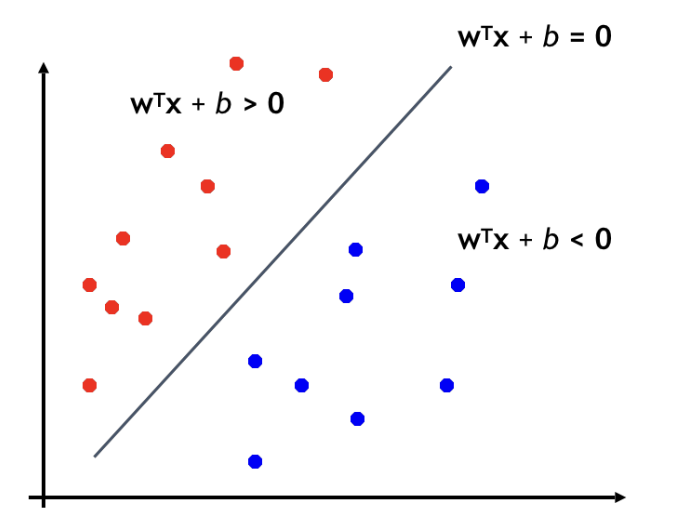
\includegraphics[width=0.4\linewidth]{Images/svm/svm_graph.png}
    \caption{Esempio di problema di classificazione binaria.}
\end{figure}

Bisogna trovare la retta $w^Tx + b$ ceh separi le due classi, ma esistono infinite rette. Va, quindi, trovata quella \textbf{ottima}. \\ 
Per fare questo, possiamo definire dei \textbf{vettori di supporto} e calcolare la loro distanza come:
\[
  r_i = \frac{w^T x_i + b}{\| w \|}
\]
\begin{figure}[!htb]
    \centering
    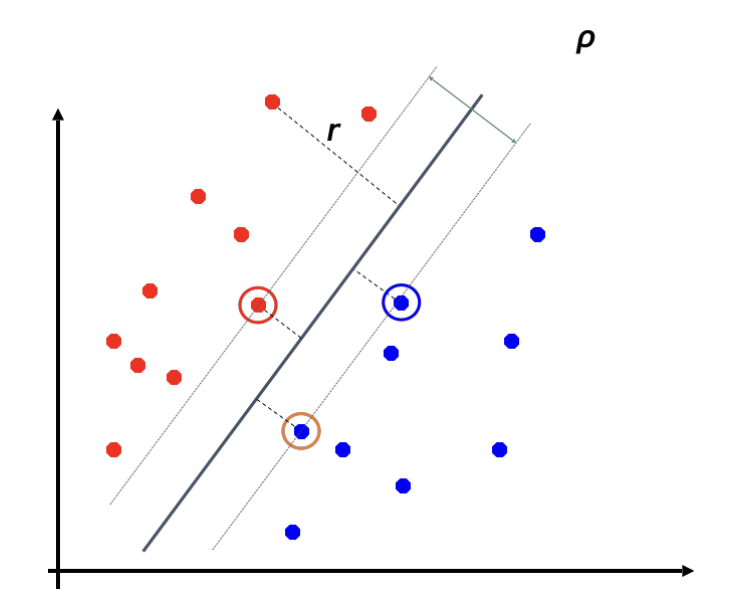
\includegraphics[width=0.4\linewidth]{Images/svm/distance.png}
    \caption{Utilizzo vettori di supporto.}
\end{figure}

L'obiettivo è massimizzare questa quantità per tutti gli $x_i$. Puntiamo al boundary che offre la maggiore sicurezza.

\begin{ex}[Calcolo dei margini]
Dato un dataset $D = (x_i, y_i)_{i \in [1, \cdots, N]}$ e $y_i \in \{-1, 1\}$ con $\rho$ come margine, vogliamo che:
\[
  y_i(w^T x_i + b) \ge \rho/2 \quad \forall x_i \in D
\]
Per il vettore di supporto $x_s$ l'equazione diventa $w^T x_s + b = \rho/2$, ottenendo quindi questa espressione per il margine:
\[
  r_s = \frac{w^T x_s + b}{\| w \|} = \frac{\rho}{2 \| w \|} = \frac{1}{\| \hat{w} \|}
\]
\[
  \rho = 2r_s = \frac{2}{\| w \|}
\]
\end{ex}

\subsection{Problema quadratico SVM}
La formula di \textbf{massimizzazione} del margine:
\[
  \arg\max_{w,b} \frac{2}{\| w \|} \quad s.t.
\]
\[
  y_i(w^T x_i + b) \ge 1 \quad \forall(x_i, y_i) \in D
\]
Equivalente a quella di \textbf{minimizzazione} dei pesi:
\[
  \arg\min_{w,b} \| w \|^2 \quad s.t.
\]
\[
  y_i(w^T x_i + b) \ge 1 \quad \forall(x_i, y_i) \in D
\]
\subsection{Ottimizzazione Vincolata}
In alcuni casi, potrebbe essere necessario ottimizzare problemi condizionati:
\[
  \min f(x)
\]
\[
  \text{subject to} \; h_i(x) \ge 0 \quad \text{for} \; i \in 1, \cdots, N
\]
\begin{defn}[Condizioni di Lagrange]
  La funzione Lagrangiana è:
  \[
    L(x, \alpha) = f(x) - \sum_{i}^N \alpha_i h_i(x) \quad \text{con} \quad \alpha_i \geq 0
  \]
  Dove:
  \begin{itemize}
    \item Se per $x_i$, $h(x_i) > 0$ allora $\alpha = 0$ il vincolo si dice \textbf{inattivo} e la soluzione è $x^* \mid \nabla f(x) = 0$
    \item Se per $x_i$, $h(x_i) = 0$ allora $\alpha > 0$ il vincolo si dice \textbf{attivo} e la soluzione è $x^* \mid \nabla f(x) - \alpha^T \nabla h(x) = 0$
  \end{itemize}
\end{defn}
Mettendo tutto insieme, troviamo le condizioni di \textbf{Karush-Kuhn-Tucker (KKT)}, che costituiscono condizioni necessarie per l'esistenza di una soluzione unica $x_*$:
\[
  \begin{aligned}
    &\nabla f(x^*) - \alpha^T \nabla h(x^*) = 0 \\
    &h(x^*) \ge 0 \\
    &\alpha_i \geq 0 \\
    &\alpha^T h(x) = 0
  \end{aligned}
\]
\subsection{Classicatore SVM}
La funzione di classificazione SVM lineare nella forma \textbf{primale}, inglobando $b$ nei pesi $w$ con una dimensione in più, è:
\[
  f(x) = w^T x
\]
Invece, nella forma \textbf{duale} è:
\[
  f(x) = \sum^N_{i=1}{a_i y_i x_i^T x}
\]
\begin{note}[Margini non separabili]
  Se i pattern dei dati non sono separabili mediante un iperpiano lineare, un insieme di \textbf{variabili di slack} $\epsilon = \epsilon_1, \epsilon_2, \cdots, \epsilon_N$ sono introdotte con $\epsilon_i \ge 0$ 
  facendo diventare i vincoli dell'SVM: 
  \[
    y_i(x_i w + b) \ge 1 - \epsilon_i
  \]
  Inoltre, il problema di ottimizzazione diventa:
  \[
    \min \frac{1}{2} \| w \|^2 + C \sum_i^N{\epsilon_i}
  \]
  \[
    \text{subject to} \; y_i(w^T x_i + b) \ge 1 - \epsilon_i \quad \text{con} \; \epsilon_i \ge 0
  \]
\end{note}

\subsection{SVM non Lineare}
Cosa succede se le classi non sono separabili linearmente?

\begin{figure}[!htb]
    \centering
    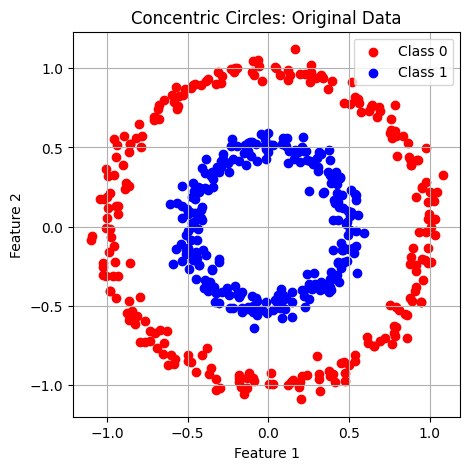
\includegraphics[width=0.3\linewidth]{Images/svm/svm_non_linear.png}
    \caption{Grafico di un SVM non lineare.}
\end{figure}

La soluzione migliore, è trasformare lo spazio di classificazione in uno in cui il confine è lineare.

\begin{figure}[!htb]
    \centering
    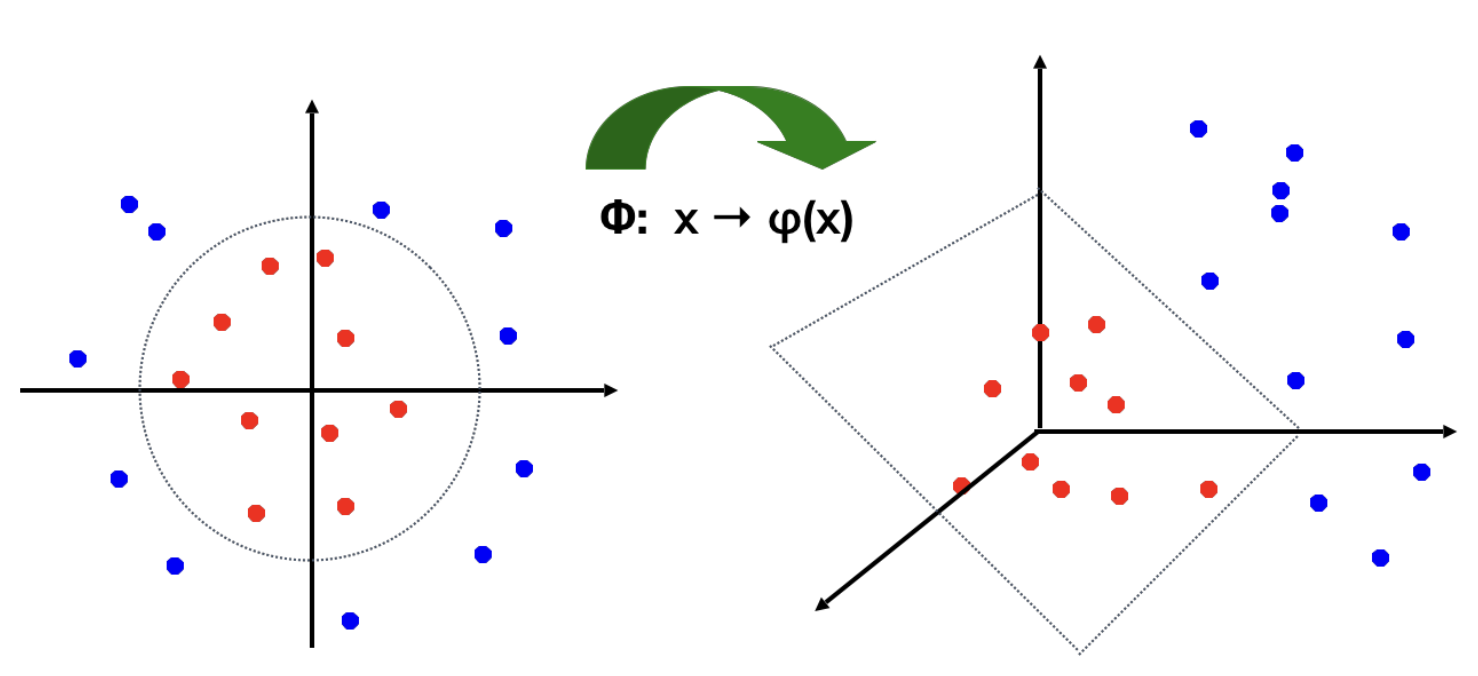
\includegraphics[width=0.45\linewidth]{Images/svm/svm_changed.png}
    \caption{Grafico sul cambio di spazio di classificazione.}
\end{figure}
Potremmo utilizzare una mappatura basata su una funzione non lineare: $\phi : x \rightarrow \phi(x)$

\newpage
\begin{defn}[Funzione di Kernel]
  Una funzione kernel mappa implicitamente i dati in uno spazio ad alta dimensionalità senza la necessità di calcolare esplicitamente ogni $\phi(x)$.
\end{defn}

\begin{ex}[Definizione funzione kernel]
  Dato $f(x) = \sum_{i=1}^N{a_i y_i (x_i^T x)}$:
  \begin{enumerate}
    \item \textbf{Mappatura non lineare:} $\phi : x \rightarrow \phi(x)$.
    \item \textbf{Definire la kernel function:} $\phi(x_i)^T\phi(x_j) = K(x_i, x_j)$.
    \item \textbf{Sostituzione:} $f(x) = \sum^N_{i=1}{a_i y_i K(x_i, x_j)}$.
  \end{enumerate}
\end{ex}

Ci sono, inoltre, vari tipi di kernel:
\begin{itemize}
  \item \textbf{Lineare:} $K(x, x_i) = x^T x_i$, utilizzato dal classificatore SVM classico.
  \item \textbf{Polinomiale:} $K(x, x_i) = (1 + x^T x_i)^p$, espande in maniera polinomiale le dimensioni come $\binom{d+p}{d}$.
  \item \textbf{RBF (Gaussiano):} $K(x, x_i) = \exp(-\frac{\| x - x_i \|^2}{2 \sigma^2})$, espande in una dimensione infinita, come $e^x = \sum_{n=1}^{\infty} \frac{x^n}{n!}$.
\end{itemize}
